\begin{figure}
    \centering
    
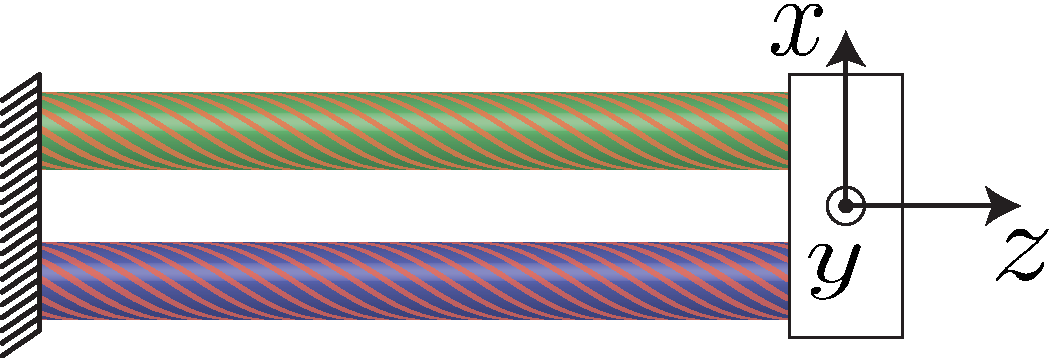
\includegraphics[width=0.6\linewidth]{figures/axesNaligned_2par.pdf}

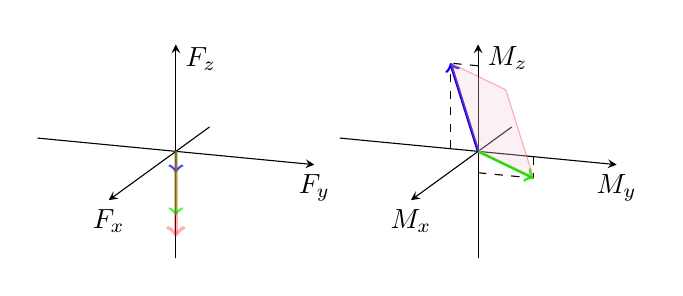
\begin{tikzpicture}
\def\scl{0.7} % define scale variable for plots

%\node[style={anchor=center}] {\includegraphics[width=0.75\linewidth]{figures/axesNaligned_2par.pdf}} at (0,2);

% PRACTICE PLOT
\matrix [row sep=0cm, column sep=0cm, style={align=center}] (my matrix) at (0,0)
{
% PRACTICE PLOT #3
\begin{axis}[
    view={110}{20},
    axis lines=center,
    % axis equal image,
    xlabel={$F_x$},
    ylabel={$F_y$},
    zlabel={$F_z$},
    ymin=-5, ymax=5, ytick={0}, %ylabel near ticks,
    xmin=-5, xmax=10, xtick={0}, %xticklabel=$\pgfmathprintnumber{\tick}^\circ$, xlabel near ticks, 
    zmin=-5, zmax=5, ztick={0}, %z dir=reverse,
    xlabel style={anchor=north}, ylabel style={anchor=north},
    scale=\scl,
    anchor=center,
    ]
    \addplot3[->, line width=1pt, blue, opacity=0.7] coordinates {(0,0,0) (0,0,-1)};
    \addplot3[->, line width=1pt, green, opacity=0.7] coordinates {(0,0,0) (0,0,-3)};
    \addplot3[->, opacity=0.3, fill=purple!20, color=red, line width=1.5pt] coordinates {(0,0,0) (0,0,-4)};
\end{axis};
&
\begin{axis}[
    view={110}{20},
    axis lines=center,
    % axis equal image,
    xlabel={$M_x$},
    ylabel={$M_y$},
    zlabel={$M_z$},
    ymin=-5, ymax=5, ytick={0}, %ylabel near ticks,
    xmin=-5, xmax=10, xtick={0}, %xticklabel=$\pgfmathprintnumber{\tick}^\circ$, xlabel near ticks, 
    zmin=-5, zmax=5, ztick={0}, %z dir=reverse,
    xlabel style={anchor=north}, ylabel style={anchor=north},
    scale=\scl,
    anchor=center,
    ]
    \def\pa{(0,2,-1)}
    \def\pb{(0,-1,4)}
    % connector lines for perspective
    \addplot3[dashed] coordinates {(0,2,0) \pa};
    \addplot3[dashed] coordinates {(0,0,-1) \pa}; 
    \addplot3[dashed] coordinates {(0,-1,0) \pb};
    \addplot3[dashed] coordinates {(0,0,4) \pb};
    % force vectors
    \addplot3[->, line width=1pt, green] coordinates {(0,0,0) \pa};
    \addplot3[->, line width=1pt, blue] coordinates {(0,0,0) \pb};
    % faces of shape
    \addplot3[patch, opacity=0.3, fill=purple!20, faceted color=red, patch type=rectangle] 
        coordinates {
                    (0,0,0) \pa (0,1,3) \pb
                    };
\end{axis};
\\
};
\end{tikzpicture}

    \caption{The force polygon for a parallel combination of 2 FREEs with fiber angles of opposite sign. For visual clarity, the force and moment components of the polygon have been plotted separately.}
    \label{fig:torque3d-2par}
\end{figure}